\documentclass[11pt,a4paper]{article}

\usepackage[margin=2.4cm]{geometry}
\usepackage{amsmath}
\usepackage{amssymb}
\usepackage{graphicx}
\usepackage{booktabs}
\usepackage{longtable}
\usepackage{array}
\usepackage{float}
\usepackage{caption}
\usepackage[table]{xcolor}
\usepackage{hyperref}
\hypersetup{colorlinks=true,linkcolor=black,citecolor=black,urlcolor=blue}

\newcommand{\degC}{\,^{\circ}\mathrm{C}}
\newcommand{\unit}[1]{\,\mathrm{#1}}

\title{\textbf{Flight Readiness Review --- Payload Thermal Analysis}\\[2mm]
\large High-Altitude Balloon Event-Camera Payload\\[1mm]
\normalsize Operating concept: on-board computer powered at 16 km}
\author{Thermal Analysis --- Systems Engineering}
\date{\today}

\begin{document}
\maketitle

\begin{abstract}
\noindent This report documents the thermal model and flight-readiness assessment of
the high-altitude balloon (HAB) event-camera payload for the operating concept in which
the on-board computer (OBC) is powered only on reaching the imaging altitude of
$16\unit{km}$. A coupled three-block model (external environment, enclosure-wall
conduction, and the two-dimensional axisymmetric internal field) is solved over the
ascent-to-apogee mission window from a cold-night initial temperature of $+5\degC$. All
seventeen payload components remain within their operating temperature limits for the
full analysed window, with a minimum cold-side operating margin of $+7.6\degC$. The
thermal design is assessed \textbf{GO} for flight.
\end{abstract}

\tableofcontents
\bigskip

% ============================================================
\section{System Description and Geometry}
% ============================================================
The payload is housed in a cylindrical expanded-polypropylene (EPP) Thermobox enclosure.
The internal cavity is modelled as an axisymmetric cylinder of internal radius $R_{int}$
and internal height $L_{int}$, surrounded by a uniform EPP wall of thickness $L_{wall}$
(side and end caps). The geometry is summarised in Table~\ref{tab:geom}.

\begin{table}[H]
\centering
\caption{Enclosure geometry.}
\label{tab:geom}
\begin{tabular}{llr}
\toprule
Symbol & Quantity & Value \\
\midrule
$R_{int}$ & Internal radius            & $0.080\unit{m}$ \\
$L_{int}$ & Internal height            & $0.250\unit{m}$ \\
$L_{wall}$& Side-wall thickness (EPP)  & $0.030\unit{m}$ \\
$L_{cap}$ & End-cap thickness (EPP)    & $0.030\unit{m}$ \\
$R_{box}$ & Outer radius               & $0.110\unit{m}$ \\
$L_{box}$ & Outer height               & $0.310\unit{m}$ \\
$D_{box}$ & Outer diameter (convection)& $0.220\unit{m}$ \\
\bottomrule
\end{tabular}
\end{table}

\begin{figure}[H]
\centering
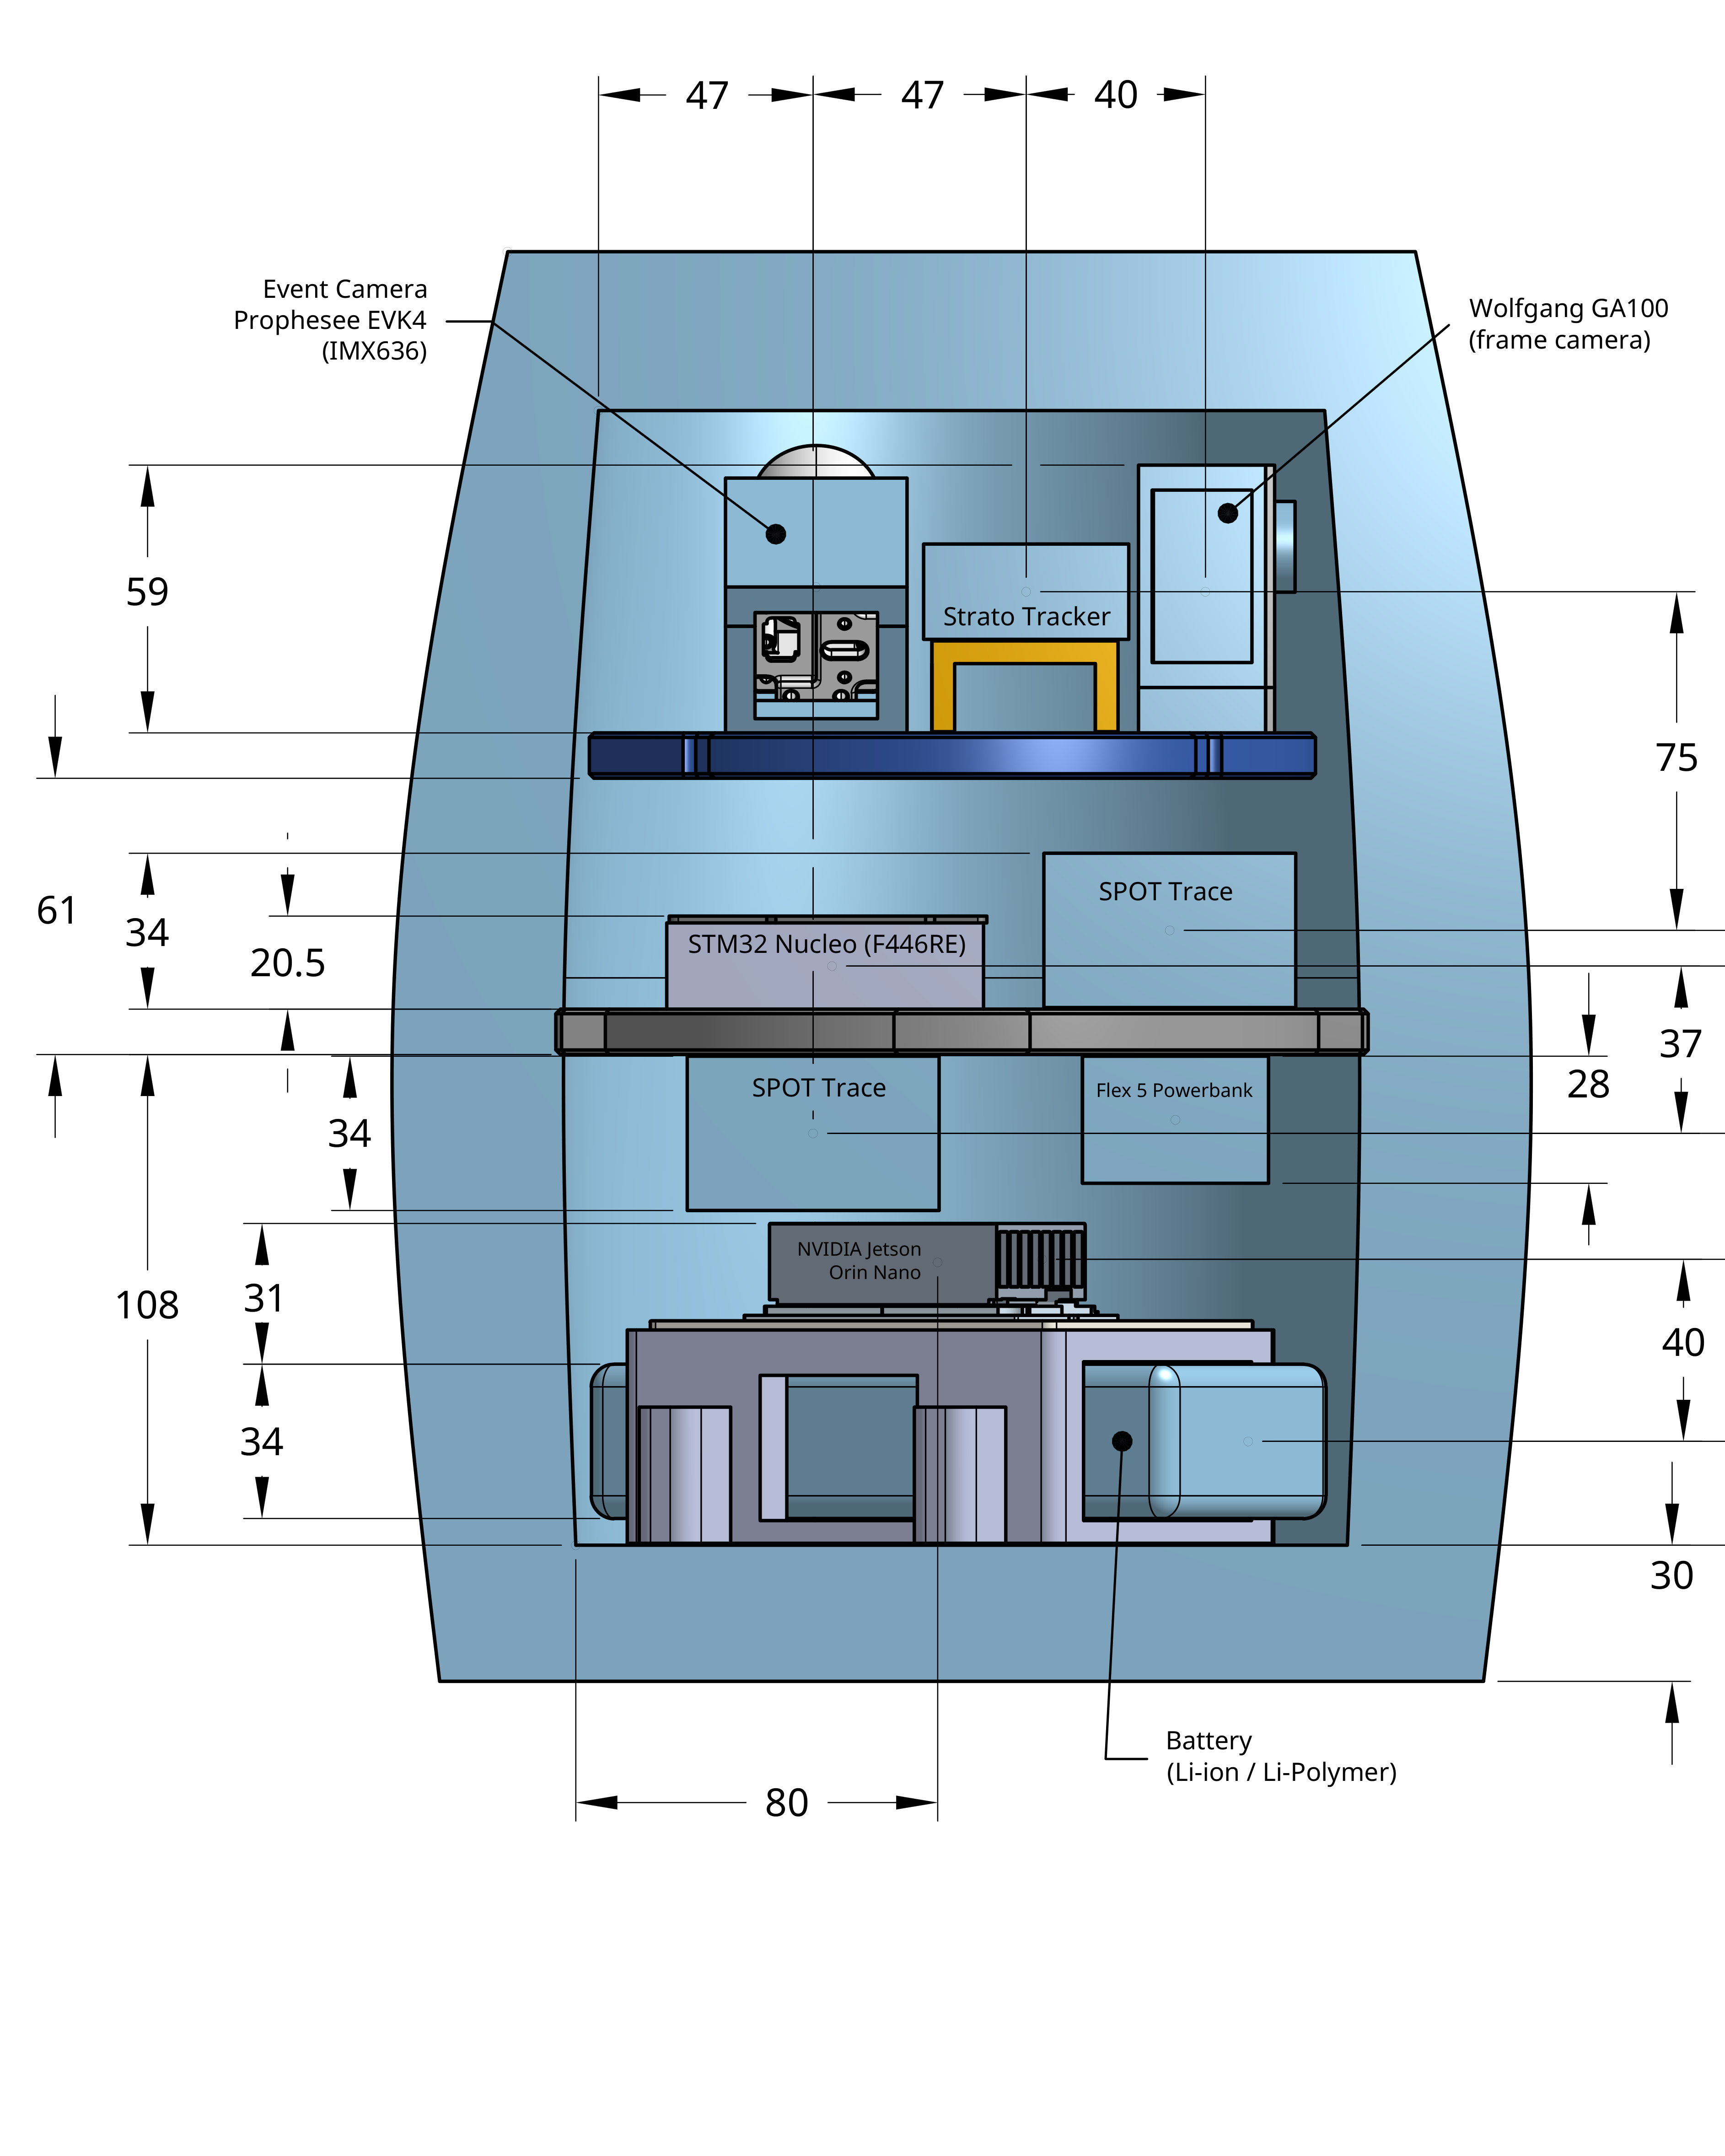
\includegraphics[width=0.62\textwidth]{cad_section.png}
\caption{Mechanical CAD section used as the reference layout for the meshed model.
The interior resolves four stacked rows: cameras and tracker on top
(EVK4 + lens, Strato Tracker, GA100), the avionics row (STM32, SPOT Trace),
the power/recovery row (GNSS/SD cluster, Flex~5 powerbank), and the heavy
bottom row (Jetson Orin Nano inboard, battery outboard, on-board storage).
Components are mounted with a clearance to the side wall.}
\label{fig:cad}
\end{figure}

% ============================================================
\section{Modelling Methodology}
% ============================================================
The model is decomposed into three coupled blocks. Block~A provides the external
free-stream temperature and convective coefficient as a function of altitude and
ascent velocity. Block~B solves transient conduction through the enclosure wall and
end caps. Block~C solves the two-dimensional axisymmetric temperature field of the
internal cavity, driven by the component heat loads and bounded by the Block~B wall
temperatures. The blocks are advanced with a lagged coupling each timestep.

% ------------------------------------------------------------
\subsection{Block A --- External Environment and Forced Convection}
% ------------------------------------------------------------
The ambient state is evaluated with the US Standard Atmosphere 1976, piecewise by
layer. Within a layer of base altitude $h_b$, base temperature $T_b$, base pressure
$P_b$ and lapse rate $L_b$,
\begin{equation}
T(h) = T_b + L_b\,(h-h_b),
\end{equation}
\begin{equation}
P(h) =
\begin{cases}
P_b\left(\dfrac{T}{T_b}\right)^{-g/(L_b R)}, & L_b \neq 0,\\[3mm]
P_b\,\exp\!\left(-\dfrac{g\,(h-h_b)}{R\,T_b}\right), & L_b = 0,
\end{cases}
\qquad
\rho = \frac{P}{R\,T},
\end{equation}
with $g=9.80665\unit{m/s^2}$ and $R=287.058\unit{J/(kg\,K)}$. Transport properties use
Sutherland-type fits,
\begin{equation}
\mu(T) = \frac{1.458\times10^{-6}\,T^{3/2}}{T+110.4},
\qquad
k_{air}(T) = \frac{2.495\times10^{-3}\,T^{0.8646}}{1 + 245.4\cdot 10^{-12/T}/T},
\qquad
\mathrm{Pr} = \frac{\mu\,c_p}{k_{air}}.
\end{equation}

The enclosure is treated as a cylinder in cross-flow at the ascent velocity $V$. The
Reynolds number and the Churchill--Bernstein Nusselt-number correlation give the
external convective coefficient:
\begin{equation}
\mathrm{Re} = \frac{\rho\,V\,D_{box}}{\mu},
\end{equation}
\begin{equation}
\mathrm{Nu} = 0.3 +
\frac{0.62\,\mathrm{Re}^{1/2}\,\mathrm{Pr}^{1/3}}
{\left[\,1+(0.4/\mathrm{Pr})^{2/3}\,\right]^{1/4}}
\left[\,1+\left(\frac{\mathrm{Re}}{282\,000}\right)^{5/8}\,\right]^{4/5},
\qquad
h_{ext} = \frac{\mathrm{Nu}\,k_{air}}{D_{box}}.
\end{equation}

% ------------------------------------------------------------
\subsection{Block B --- One-Dimensional Wall Conduction}
% ------------------------------------------------------------
Each wall (side, top cap, bottom cap) is discretised into $N$ nodes across the
thickness, with spacing $\Delta x = L_{wall}/(N-1)$. Transient conduction is advanced
with implicit Euler in a finite-volume form. Boundary nodes carry half control volumes;
interior nodes carry full control volumes. The outer surface (node $0$) exchanges with
the atmosphere through $h_{ext}$ and the inner surface (node $N-1$) with the cavity air
through the internal coefficient $h_{int}$:
\begin{align}
\text{Outer:}\quad &
\frac{\rho c_p \tfrac{\Delta x}{2}}{\Delta t}\left(T_0^{n+1}-T_0^{n}\right)
= h_{ext}\left(T_\infty - T_0^{n+1}\right) + \frac{k}{\Delta x}\left(T_1^{n+1}-T_0^{n+1}\right),\\[1mm]
\text{Interior:}\quad &
\frac{\rho c_p \Delta x}{\Delta t}\left(T_i^{n+1}-T_i^{n}\right)
= \frac{k}{\Delta x}\left(T_{i-1}^{n+1}-2T_i^{n+1}+T_{i+1}^{n+1}\right),\\[1mm]
\text{Inner:}\quad &
\frac{\rho c_p \tfrac{\Delta x}{2}}{\Delta t}\left(T_{N-1}^{n+1}-T_{N-1}^{n}\right)
= \frac{k}{\Delta x}\left(T_{N-2}^{n+1}-T_{N-1}^{n+1}\right) + h_{int}\left(T_{air}-T_{N-1}^{n+1}\right).
\end{align}
These equations form a tridiagonal system solved directly each timestep. The camera
optical windows are modelled as a thin glass pane solved with the same one-dimensional
scheme and coupled to the internal field as a parallel conductance on the upper ring.

The internal coefficient $h_{int}$ represents natural convection of the cavity air.
In the laminar enclosure regime the Nusselt number scales as
$\mathrm{Nu}\propto\mathrm{Ra}^{1/4}$, and since $\mathrm{Ra}\propto\rho^{2}\propto P^{2}$
the coefficient varies with the square root of the local ambient pressure $P(h)$ from
Block~A:
\begin{equation}
h_{int}(h) = h_{int,0}\,\sqrt{\frac{P(h)}{P_0}},
\qquad h_{int,0}=1.5\unit{W/(m^2 K)},\quad P_0 = 101{,}325\unit{Pa}.
\end{equation}
As the payload ascends and the atmosphere thins, the internal convective coupling
weakens accordingly, decreasing from $1.5\unit{W/(m^2 K)}$ at the surface to
approximately $0.14\unit{W/(m^2 K)}$ near apogee.

% ------------------------------------------------------------
\subsection{Block C --- Two-Dimensional Axisymmetric Internal Field}
% ------------------------------------------------------------
The cavity is meshed on a uniform $(r,z)$ grid with cell centres at
$r_i=(i+\tfrac12)\Delta r$ and $z_j=(j+\tfrac12)\Delta z$. For cell $i$ the radial faces
lie at $r_i^- = i\,\Delta r$ and $r_i^+ = (i+1)\Delta r$, giving the face areas and cell
volume
\begin{equation}
A_{r}^{-} = 2\pi r_i^{-}\,\Delta z,\qquad
A_{r}^{+} = 2\pi r_i^{+}\,\Delta z,\qquad
A_{z} = \pi\!\left(r_i^{+2}-r_i^{-2}\right),\qquad
V = A_z\,\Delta z .
\end{equation}
Each cell $P$ is advanced with an implicit finite-volume energy balance over its faces
$f$ to neighbours $F$, with an internal source $Q_P$ (the component dissipation assigned
to the cell):
\begin{equation}
\frac{\rho_P c_{p,P} V_P}{\Delta t}\left(T_P^{n+1}-T_P^{n}\right)
= \sum_{f} G_f\left(T_F^{n+1}-T_P^{n+1}\right) + Q_P .
\end{equation}
Interface conductances use the harmonic-mean conductivity to handle dissimilar
materials,
\begin{equation}
G_f = \frac{k_{harm}\,A_f}{d},\qquad
k_{harm} = \frac{2\,k_P\,k_F}{k_P+k_F},
\end{equation}
where $d=\Delta r$ for radial faces and $d=\Delta z$ for axial faces. Dirichlet
boundaries (the inner wall ring $T_{r,wall}(z)$ from the side wall, and the cap
temperatures $T_{top}$, $T_{bot}$) use a half-cell distance $d/2$, contributing
$G_{bc}=k\,A_f/(\Delta r/2)$ to the diagonal and $G_{bc}\,T_{bc}$ to the right-hand side.
The axis ($i=0$) is a symmetry boundary with zero radial flux ($A_r^{-}=0$). On the
upper ring the glass window adds a parallel path of area $A_{win}$ to $T_{window}$
alongside the wall area $A_{eps}$ to $T_{r,wall}$. Assembling all cells yields a sparse
linear system $\mathbf{A}\,\mathbf{T}^{n+1}=\mathbf{b}$, solved with a sparse direct
solver each timestep.

% ------------------------------------------------------------
\subsection{Coupling}
% ------------------------------------------------------------
Per timestep $n$: (i) Block~A returns $T_\infty$, $h_{ext}$ and the ambient pressure
from the altitude and velocity profiles; (ii) the cavity air temperature $T_{air}$ is
taken as the volume-weighted mean of the air cells and $h_{int}$ is evaluated at the
current altitude; (iii) Block~B advances the side wall, caps and window pane; (iv)
Block~C advances the internal field using the updated inner-surface temperatures. The
numerical parameters are listed in Table~\ref{tab:num}.

\begin{table}[H]
\centering
\caption{Numerical and boundary parameters.}
\label{tab:num}
\begin{tabular}{llr}
\toprule
Symbol & Quantity & Value \\
\midrule
$N_r \times N_z$ & Internal mesh           & $32 \times 100$ (3200 cells) \\
$\Delta r,\ \Delta z$ & Cell size          & $2.5\unit{mm}$ \\
$N$ & Wall nodes (Block B)                 & $5$ \\
$\Delta t$ & Timestep (implicit)           & $30\unit{s}$ \\
$t_{end}$ & Analysis window               & $6800\unit{s}$ ($113.3$ min) \\
$h_{int,0}$ & Internal coefficient (sea level) & $1.5\unit{W/(m^2 K)}$ \\
$T_{launch}$ & Initial temperature        & $278.15\unit{K}$ ($5\degC$) \\
\bottomrule
\end{tabular}
\end{table}

% ============================================================
\section{Component Database}
% ============================================================
The payload comprises seventeen entries (Table~\ref{tab:db}). Each is mapped to a
rectangular cell region of the mesh per the CAD layout (Fig.~\ref{fig:cad}), assigned an
effective material, a steady electrical dissipation, and operating temperature limits.
Storage devices (SSD, USB) dissipate their drawn power as heat.

\begin{longtable}{p{4.6cm} l r r r r}
\caption{Payload component database: material, mass, steady dissipation, and operating
temperature limits.}\label{tab:db}\\
\toprule
Component & Subsys. & $m$ [g] & $P$ [W] & $T_{op,min}$ & $T_{op,max}$ \\
\midrule
\endfirsthead
\multicolumn{6}{c}{\tablename\ \thetable\ -- continued}\\
\toprule
Component & Subsys. & $m$ [g] & $P$ [W] & $T_{op,min}$ & $T_{op,max}$ \\
\midrule
\endhead
\midrule \multicolumn{6}{r}{continued on next page}\\
\endfoot
\bottomrule
\endlastfoot
NVIDIA Jetson Orin Nano        & OBC      & 260 & 7.00 & $-25\degC$ & $90\degC$ \\
Battery (Li-ion / Li-Po)       & EPS      & 1000& 0.30 & $-20\degC$ & $60\degC$ \\
250 GB SSD (NVMe M.2)          & OBC      & 10  & 3.00 & $-40\degC$ & $85\degC$ \\
USB Stick (USB 3.0)            & OBC      & 5   & 3.00 & $-25\degC$ & $85\degC$ \\
STM32 Nucleo F446RE            & OBC      & 50  & 0.30 & $-40\degC$ & $85\degC$ \\
GNSS Module (u-blox NEO-M9N)   & Sensors  & 10  & 0.15 & $-40\degC$ & $85\degC$ \\
SD Card Reader + Card          & OBC      & 5   & 0.05 & $-25\degC$ & $85\degC$ \\
IMU (TDK ICM-20948) $\times2$  & Sensors  & 5   & 0.01 & $-40\degC$ & $85\degC$ \\
Env. Sensor MS8607 $\times2$   & Sensors  & 2   & 0.005& $-40\degC$ & $85\degC$ \\
SPOT Trace                     & Recovery & 70  & 0.30 & $-40\degC$ & $60\degC$ \\
Strato Tracker                 & Recovery & 60  & 0.50 & $-40\degC$ & $85\degC$ \\
Flex 5 Powerbank               & EPS      & 400 & 0.40 & $-10\degC$ & $45\degC$ \\
Wolfgang GA100 (frame camera)  & Payload  & 120 & 3.00 & $-10\degC$ & $40\degC$ \\
Prophesee EVK4 (IMX636)        & Payload  & 130 & 1.50 & $-20\degC$ & $60\degC$ \\
Soyo C-Mount Lens              & Payload  & 50  & 0.00 & $-40\degC$ & $85\degC$ \\
GNSS Antenna (ceramic patch)   & Sensors  & 20  & 0.00 & $-40\degC$ & $85\degC$ \\
Wiring \& Connectors           & EPS      & 200 & 0.50 & $-55\degC$ & $125\degC$ \\
\end{longtable}

\begin{figure}[H]
\centering

\includegraphics[width=0.92\textwidth]{mesh_map.png}
\caption{Compiled materials map (left) and heat-source map (right), shown in CAD
orientation ($z$ vertical, full mirrored diameter). The map reproduces the four-row
layout of Fig.~\ref{fig:cad}; the source map shows the Jetson as the dominant internal
heat source in the bottom row.}
\label{fig:mesh}
\end{figure}

% ============================================================
\section{Mission Profile}
% ============================================================
The analysed window is the powered ascent from launch to apogee and the first part of
descent. The balloon ascends at $5\unit{m/s}$ to a burst altitude of $33\unit{km}$
($t=6600\unit{s}$), then descends under parachute at $5.5\unit{m/s}$. The imaging
altitude of $16\unit{km}$ is reached at $t\approx3200\unit{s}$ ($53.5$ min). In this
operating concept the OBC (Jetson Orin Nano, $7\unit{W}$) is held unpowered during
ascent and is energised on reaching $16\unit{km}$, remaining active for the one-hour
imaging window to the end of the analysis ($t=6800\unit{s}$); all other payload loads
are active from launch. The resulting free-stream temperature and external convective
coefficient are shown in Fig.~\ref{fig:env}: the ambient reaches the tropopause minimum
near $-56.5\degC$, while $h_{ext}$ falls monotonically with the thinning atmosphere.

\begin{figure}[H]
\centering

\includegraphics[width=0.9\textwidth]{environment.png}
\caption{External environment over the mission window: altitude, free-stream
temperature $T_\infty$, and external convective coefficient $h_{ext}$ from Block~A.}
\label{fig:env}
\end{figure}

% ============================================================
\section{Results}
% ============================================================
The internal temperature field is shown at five instants in Fig.~\ref{fig:contour}.
The cavity cools through the ascent with no internal heat source until the OBC is
energised at $16\unit{km}$, after which the Jetson establishes a warm core in the bottom
row. Component temperature histories are given in Fig.~\ref{fig:traces}, and the
minima/maxima with cold-side operating margins are tabulated in
Table~\ref{tab:results}.

\begin{figure}[H]
\centering

\includegraphics[width=0.96\textwidth]{temperature_contour.png}
\caption{Internal temperature field (CAD orientation, full diameter) at five mission
times. With the OBC unpowered during ascent the cavity tracks the cooling wall; the
warm bottom-row core appears only after the OBC is energised at $16\unit{km}$.}
\label{fig:contour}
\end{figure}

\begin{figure}[H]
\centering

\includegraphics[width=0.92\textwidth]{component_temperatures.png}
\caption{Component mean-temperature histories over the mission window with operating
limit bands.}
\label{fig:traces}
\end{figure}

\begin{table}[H]
\centering
\caption{Component temperature results over the analysis window and cold-side operating
margin $\Delta T = T_{min}-T_{op,min}$. All components are within limits.}
\label{tab:results}
\begin{tabular}{p{5.0cm} r r r r c}
\toprule
Component & $T_{min}$ & $T_{max}$ & $T_{op,min}$ & $\Delta T$ & Status \\
\midrule
NVIDIA Jetson Orin Nano        & $\phantom{0}5.0$ & $19.0$ & $-25$ & $+30.0$ & OK \\
Battery (Li-ion / Li-Po)       & $\phantom{0}3.4$ & $\phantom{0}7.4$ & $-20$ & $+23.4$ & OK \\
250 GB SSD (NVMe M.2)          & $\phantom{0}5.0$ & $27.1$ & $-40$ & $+45.0$ & OK \\
USB Stick (USB 3.0)            & $\phantom{0}5.0$ & $21.7$ & $-25$ & $+30.0$ & OK \\
STM32 Nucleo F446RE            & $\phantom{0}3.8$ & $\phantom{0}8.3$ & $-40$ & $+43.8$ & OK \\
GNSS Module (u-blox NEO-M9N)   & $\phantom{0}5.0$ & $\phantom{0}9.5$ & $-40$ & $+45.0$ & OK \\
SD Card Reader + Card          & $\phantom{0}4.8$ & $\phantom{0}9.0$ & $-25$ & $+29.8$ & OK \\
IMU (TDK ICM-20948) $\times2$  & $\phantom{0}5.0$ & $\phantom{0}9.8$ & $-40$ & $+45.0$ & OK \\
Env. Sensor MS8607 $\times2$   & $\phantom{0}5.0$ & $\phantom{0}9.4$ & $-40$ & $+45.0$ & OK \\
SPOT Trace                     & $-0.7$ & $\phantom{0}6.7$ & $-40$ & $+39.3$ & OK \\
Strato Tracker                 & $\phantom{0}5.0$ & $18.8$ & $-40$ & $+45.0$ & OK \\
Flex 5 Powerbank               & $-0.8$ & $\phantom{0}6.6$ & $-10$ & $\phantom{0}+9.2$ & OK \\
Wolfgang GA100 (frame camera)  & $-2.4$ & $10.6$ & $-10$ & $\phantom{0}+7.6$ & OK \\
Prophesee EVK4 (IMX636)        & $\phantom{0}5.0$ & $13.7$ & $-20$ & $+25.0$ & OK \\
Soyo C-Mount Lens              & $\phantom{0}1.9$ & $10.6$ & $-40$ & $+41.9$ & OK \\
GNSS Antenna (ceramic patch)   & $-2.1$ & $\phantom{0}6.9$ & $-40$ & $+37.9$ & OK \\
Wiring \& Connectors           & $-1.6$ & $\phantom{0}6.4$ & $-55$ & $+53.4$ & OK \\
\bottomrule
\end{tabular}
\end{table}

All temperatures are in $\degC$. The minimum operating margin across the payload is
$+7.6\degC$ on the Wolfgang GA100 frame camera, the most cold-limited unit
($T_{op,min}=-10\degC$), which is mounted in the top-outer corner and is therefore the
most exposed to the cold side wall and top cap. The Flex~5 powerbank is the second most
constrained unit at $+9.2\degC$. On the hot side, the warmest component is the SSD at
$27.1\degC$ against an $85\degC$ limit and the Jetson peaks at $19.0\degC$ against
$90\degC$; hot-side margins therefore exceed $50\degC$ throughout.

% ============================================================
\section{Conclusion}
% ============================================================
The coupled three-block thermal model, built directly on the mechanical CAD layout,
shows that with the OBC powered at $16\unit{km}$ all seventeen payload components remain
within their operating temperature limits throughout the powered ascent-to-apogee
window from a $+5\degC$ initial temperature, with a minimum cold-side margin of
$+7.6\degC$. On this basis the payload thermal design is assessed
\textbf{GO for flight}.

\end{document}
